\section{Experimentierumgebung}
Das folgende Kapitel verdeutlicht den Aufbau der Experimentierumgebung, die für die technische Durchführung benötigt wurde. Dabei wird auf Datensätze, Modelle und deren Strukturen, wie auch auf die Implementierung von Angriffsmethoden und Verteidigungsmaßnahmen eingegangen. Die Auswahl und Konfiguration dieser Elemente sind entscheidend für die Reproduzierbarkeit der Experimente sowie für die Validität und Aussagekraft der ausgearbeiteten Ergebnisse.
\subsection{Datensätze}
%mnist
%celeba
%ffhq
In diesem Abschnitt werden die Datensätze vorgestellt, die als Grundlage für die Trainings- und Angriffsdurchführungen in dieser Forschungsarbeit dienen. Eine sorgfältige Auswahl und detaillierte Beschreibung dieser Datensätze sind von zentraler Bedeutung, um die Integrität der Experimente zu gewährleisten und eine solide Grundlage für die Analyse der Ergebnisse und Beobachtungen zu schaffen.

In dieser Arbeit wurde aus Gründen der Einfachheit der MNIST-Datensatz (\cite{noauthor_mnist_nodate}) verwendet, welcher eine präzise Abfolge von Ziffern repräsentiert. Dieser Datensatz umfasst verschiedene Datenpunkte, die den Klassen der Zahlen 0 bis 9 zugeordnet sind. 

\begin{figure}[H]
	\centering
	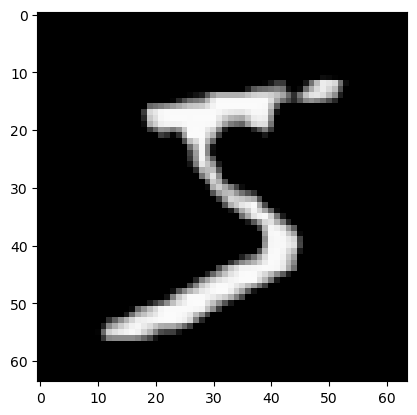
\includegraphics[width=0.2\linewidth]{Bilder/5_mnist.png}
	\caption{Beispielbild des MNIST-Datensatzes}
	\label{img:mnist}
\end{figure}

Die Datenpunkte sind in Form von sogenannten Ein-Kanal-Bildern repräsentiert, die vom menschlichen Auge in bestimmten Darstellungen als schwarz-weiß wahrgenommen werden (siehe Bild \ref{img:mnist}). Die Größe der Bilder, die zur Erstellung des Trainingsdatensatzes verwendet wurde, beträgt $64 \times 64$ Pixel. Dabei besitzt jeder Pixel einen normalisierten Wert zwischen 0 und 1, der die \glqq Farbe\grqq{} festlegt. Mit der Zusammensetzung aller Pixel entsteht das finale Bild.

Die Entscheidung für den MNIST-Datensatz wurde aufgrund seiner weiten Verbreitung in der Forschung und seiner klaren Struktur zur Repräsentation von Ziffern getroffen, wobei die Bildmerkmale vergleichsweise als \glqq einfach\grqq{} gelten. Die Fokussierung auf Zahlen im Bereich von 0 bis 9 ermöglicht eine gezielte Untersuchung spezifischer Klassen und vereinfacht die Interpretation der Ergebnisse. Dies erleichtert eine anschaulichere Analyse der durchgeführten Angriffe und liefert dem Betrachter klare und eindeutige Ergebnisse.

Der MNIST-Datensatz eignet sich besonders gut für die Evaluierung von Angriffen aufgrund seiner klaren Struktur und begrenzten Klassenanzahl. Dies ermöglicht eine präzise Bewertung der Wirksamkeit von Verteidigungsmaßnahmen und bietet gleichzeitig eine klare Vergleichsbasis für verschiedene Angriffsszenarien. Darüber hinaus hat sich gezeigt, dass auch komplexe Modelle wie das VGG16-Netzwerk auf Basis des MNIST-Datensatzes effizient trainiert werden können und bereits nach wenigen Epochen eine bemerkenswert hohe Genauigkeit auf Testdaten aufweisen.

Im Kontext neuronaler Netzwerke, die für die Generierung von Bildern eingesetzt werden, offenbart sich, dass diese rasch auf Grundlage des MNIST-Datensatzes angepasst werden können. Diese Modelle generieren zügig Bilder, die eine deutliche Ähnlichkeit zum Trainingsdatensatz aufweisen. Neben den zuvor erwähnten Gründen stellt die Veranschaulichung von Angriffen einen weiteren relevanten Aspekt für die Nutzung dieses Datensatzes dar. Aufgrund der als \glqq einfach\grqq{} geltenden Struktur der Bilder lässt sich zügig ein Vergleich zwischen Angriffen auf verschiedene Modelle herstellen, was die klare Veranschaulichung der Ergebnisse ermöglicht. Diese \glqq Einfachheit\grqq{} erweist sich als vorteilhaft für die transparente und effektive Analyse unterschiedlicher Angriffsstrategien sowie deren Auswirkungen auf die Bildgenerierung neuronaler Netzwerke.

Neben dem MNIST- wurde auch der CelebA-Datensatz (\cite{noauthor_celeba_nodate}) verwendet, der verschiedene Gesichtsbilder von 10.177 berühmten Personen in verschiedenen Klassen beinhaltet. Insgesamt hat er damit über 200.000 Bilder. Dieser eignet sich für verschiedene Use-Cases, wobei er in diesem Fall lediglich als Trainingsdatensatz für einen \glqq Personen\grqq-Klassifikator genutzt wurde. Auch hier werden die Bilder während des Ladens auf eine Größe von $64 \times 64$ Pixeln verändert und entstehen im Gegensatz zu den MNIST-Bildern aus 3 Kanälen. Auch hier wird jeder dieser Pixel auf einen normalisierten Wert zwischen 0 und 1 transformiert. Dabei wird jeweils rot, grün und blau von einem bestimmten Kanal repräsentiert. 

Der CelebA-Datensatz wurde als Vergleichsdatensatz zum zuvor genannten MNIST-Datensatz ausgewählt. Dies geschah sowohl, um Angriffe auf komplexere Datensätze zu prüfen, als auch, um Black-Box-Angriffe basierend auf einen bezüglich des CelebA-Datensatz trainierten Klassifizierer auf Grundlage eines anderen Gesichtsdatensatzes (\cite{noauthor_nvlabsffhq-dataset_2023}) zu erforschen. Diese Entscheidung ermöglichte die Simulation verschiedener Angriffsszenarien, die diverse Strategien und Durchführungsprozesse umfassen.

%hier noch ein Bild einfügen

Die Auswahl des CelebA-Datensatzes ermöglichte eine erweiterte Untersuchung der Robustheit von Modellen gegenüber Angriffen, insbesondere auf dem Gebiet der Gesichtsbilderkennung. Die Verwendung von CelebA erlaubte nicht nur die Erweiterung des Anwendungsbereichs auf komplexere und realistischere Bilder, sondern ermöglichte auch eine generalisiertere Beurteilung der Sicherheitsmechanismen. Hierbei wurde der Fokus auf die Diversität von Gesichtsmerkmalen und -attributen gelegt, um die Widerstandsfähigkeit gegenüber unterschiedlichen Angriffsdurchführungen zu prüfen.

Die vielseitige Nutzung des CelebA-Datensatzes erstreckte sich über verschiedene Trainingsparadigmen. Einerseits wurde der Datensatz zur Schulung von Klassifikatoren herangezogen, die auf der VGG16-Architektur basierten. Andererseits wurde er auch für das Training eines herkömmlichen DCGAN-Netzwerks verwendet, um die Generierung von \glqq neuen\grqq{} Gesichtsbildern zu ermöglichen. Dies ermöglichte die Evaluierung der Anfälligkeit von Modellen unterschiedlicher Architekturen gegenüber Angriffen und trug zur Erweiterung des Verständnisses für die Sicherheit von Gesichtsdatensätzen bei.
\subsection{Modelle}
%VGG16
%DCGAN
%StyleGAN
Die Architektur der eingesetzten Modelle spielt eine zentrale Rolle in der Experimentierumgebung. Hier werden die gewählten Modelle hinsichtlich ihrer Struktur und Hyperparameter, die während des Traininsprozesses verwendet wurde, detailliert beschrieben. Eine genaue Vorstellung der Modelle ist entscheidend, um nachvollziehen zu können, wie diese auf die Datensätze angewendet wurden und welche Rolle sie in den folgenden Angriffs- und Verteidigungsszenarien spielen.
\subsection{Angriffsmethoden}
%KEDMI
%RBMI
Dieser Abschnitt beleuchtet die implementierten Angriffsmethoden, die darauf abzielen, die Integrität und Sicherheit der Modelle zu kompromittieren. Die Wahl der Angriffsvektoren, deren Ausführung und Auswirkungen werden systematisch erläutert. Zusätzlich werden mögliche Schwächen der Modelle aufgezeigt, die durch die Angriffsmethoden ausgenutzt wurden. Die detaillierte Beschreibung ermöglicht es, die Reproduzierbarkeit der Angriffe zu gewährleisten und die Robustheit der Modelle zu bewerten.
\subsection{Verteidigungsmaßnahmen}
%Differential Privacy
Um den experimentellen Rahmen abzurunden, werden in diesem Abschnitt die implementierten Verteidigungsmaßnahmen präsentiert. Dies beinhaltet Schutzmechanismen, die darauf abzielen, Modelle gegen Angriffe zu stärken und ihre Robustheit zu verbessern. Die Wirksamkeit dieser Verteidigungsstrategien wird kritisch betrachtet, und es werden etwaige Limitationen oder Trade-offs diskutiert.

Die detaillierte Darstellung dieser Elemente bildet das Fundament für die nachfolgenden Experimente und ermöglicht es, die Ergebnisse in einem klaren Kontext zu interpretieren. Die sorgfältige Auswahl und Konfiguration der Experimentierumgebung ist entscheidend für die Zuverlässigkeit und Aussagekraft der gesamten Forschungsarbeit.